%\documentclass[pra,showpacs,showkeys,amsfonts,amsmath,twocolumn]{revtex4}
\documentclass[amsmath,blue]{beamer}
%\documentclass[pra,showpacs,showkeys,amsfonts]{revtex4}

\usepackage{beamerthemeshadow}
%\usepackage[dark]{beamerthemesidebar}
%\usepackage[headheight=24pt,footheight=12pt]{beamerthemesplit}
%\usepackage{beamerthemesplit}
%\usepackage[bar]{beamerthemetree}
\usepackage{graphicx}
\usepackage{pgf}

%\RequirePackage[german]{babel}
%\selectlanguage{german}
%\RequirePackage[isolatin]{inputenc}

\pgfdeclareimage[height=0.5cm]{logo}{tu-logo}
\logo{\pgfuseimage{logo}}
\beamertemplatetriangleitem
\begin{document}

\title{\bf Some remarks on digital space}
%\subtitle{Naturwissenschaftlich-Humanisticher Tag am BG 19\\Weltbild und Wissenschaft\\http://tph.tuwien.ac.at/\~{}svozil/publ/2005-BG18-pres.pdf}
%\subtitle{http://www.arxiv.org/abs/quant-ph/0406014}
\author{Karl Svozil}
\institute{Institut f\"ur Theoretische Physik, University of Technology Vienna, \\
Wiedner Hauptstra\ss e 8-10/136, A-1040 Vienna, Austria\\
svozil@tuwien.ac.at
%{\tiny Disclaimer: Die hier vertretenen Meinungen des Autors verstehen sich als Diskussionsbeitr�ge und decken sich nicht notwendigerweise mit den Positionen der Technischen Universit�t Wien oder deren Vertreter.}
}
\date{May 13, 2005}
\maketitle

%\frame[shrink=2]{\tableofcontents}



\section{Intrinsic-extrinsic observers}
\subsection{``History''}

\frame[shrink=2]{
\frametitle{(Incomplete) History}

\begin{itemize}
\item<+->
Archimedes conceived {\em ``points  outside the world, from which one could move the earth.''}

\item<+->
The 18'th century physicist B. J. Boscovich  realised that
it is not possible to measure motions or transformations if the whole
world, including all measurement apparata and observers therein, becomes
equally affected by these motions or transformations.

\item<+->
T. Toffoli,
{\sl The role of the observer in uniform systems}, in {\sl Applied
General Systems Research}, ed. by G. Klir (Plenum Press, New York,
London, 1978).

\item<+->
H. Putnam's  brain-\-in-\-a-\-vat analysis around 1980

\item<+->
K. Svozil (around 1984---) extrinsic/intrinsic difference in relativistic context, later modelling of
computational complementarity by quantum-type automata and generalized urn models

\item<+->
O. R\"ossler: Endo/Exophysics


\item<+-> Many artist; e.g.,
Daniel F. Galouye,
``Simulacron 3'' (1964), ``Total Recall,'' ``The Matrix,'' ``Waking lives,'' $\ldots$

\end{itemize}
 }

\subsection{Concepts}
\frame{
\frametitle{ }

\begin{itemize}
\item<+->
The
 {\em intrinsic}
 {\em (endo\-phy\-sics)}
 concept, is related to the question of how
 a mathematical or a logical or an algorithmic  universe
 is perceived   from within.
 The physical universe, by definition, can be perceived
 from within only.

\item<+->
The
 {\em extrinsic}
 {\em (exo\-phy\-sics)}
 concept, is related to the question of how
 a mathematical or a logical or an algorithmic  universe
 is perceived   from the outside.

\item<+->
Interface design and duality: what if we were ``the dead on vacation?''
(cf. Godard)

\end{itemize}
 }


\section{Computational complementarity}
\subsection{Example}

\frame[shrink=2]{
\begin{figure}
\begin{center}
\unitlength=0.6mm
\special{em:linewidth 0.4pt}
\linethickness{0.4pt}
\begin{picture}(150.00,71.00)
\put(21.00,46.00){\framebox(121.00,16.00)[cc]{experimenter}}
\put(21.00,11.00){\framebox(121.00,15.00)[cc]{automaton}}
\put(35.00,46.00){\vector(0,-1){19.00}}
\put(122.00,26.67){\vector(0,1){18.00}}
\put(39.00,36.00){\makebox(0,0)[lc]{input}}
\put(102.00,35.00){\makebox(0,0)[lc]{output}}
\put(15.00,7.00){\framebox(135.00,64.00)[cc]{}}
\put(95.00,65.00){\makebox(0,0)[lb]{``meta''-automaton}}
\end{picture}
\end{center}
\caption{Schematic diagram of an experiment on a single automaton,
 both taking place in a ``meta''-automaton.
 \label{f-s-experiment}}
\end{figure}
 }

\frame[shrink=2]{
 \begin{figure}
\begin{center}
\unitlength=0.650mm
\special{em:linewidth 0.4pt}
\linethickness{0.4pt}
\begin{picture}(140.00,100.00)
\put(10.00,10.00){\framebox(130.00,90.00)[cc]{}}
\put(17.00,17.00){\framebox(80.00,50.00)[cc]{}}
\put(23.00,23.00){\framebox(40.00,20.00)[cc]{}}
\put(27.00,27.00){\framebox(17.00,8.00)[cc]{}}
\put(29.00,29.00){\framebox(7.00,3.00)[cc]{}}
\put(30.00,30.00){\framebox(3.00,1.00)[cc]{}}
\put(30.00,30.00){\rule{2.00\unitlength}{1.00\unitlength}}
\put(115.00,17.00){\framebox(21.00,76.00)[cc]{{\Large exp.}}}
\put(78.00,23.00){\framebox(16.00,39.00)[cc]{exp.}}
\put(52.00,27.00){\framebox(9.00,12.00)[cc]{{\small exp.}}}
\put(39.00,29.00){\framebox(3.00,4.00)[cc]{{\tiny exp.}}}
\put(34.00,30.00){\framebox(1.00,1.00)[cc]{}}
\put(34.00,31.00){\vector(-1,0){1.00}}
\put(33.00,30.00){\vector(1,0){1.00}}
\put(36.00,29.00){\vector(1,0){3.00}}
\put(39.00,31.00){\vector(-1,0){3.00}}
\put(44.00,28.00){\vector(1,0){8.00}}
\put(52.00,34.00){\vector(-1,0){8.00}}
\put(63.00,29.00){\vector(1,0){15.00}}
\put(78.00,41.00){\vector(-1,0){15.00}}
\put(97.00,20.00){\vector(1,0){18.00}}
\put(115.00,64.00){\vector(-1,0){18.00}}
\put(42.00,84.00){\makebox(0,0)[cc]{{\Large system}}}
\put(38.00,55.00){\makebox(0,0)[cc]{system}}
\put(32.00,38.00){\makebox(0,0)[cc]{{\small system}}}
\put(31.00,33.00){\makebox(0,0)[cc]{{\tiny system}}}
\end{picture}
\end{center}
\caption{ Hierarchy of intrinsic perception.
 \label{l.fiss}}
\end{figure}
 }

\frame[shrink=2]{
\begin{figure}
\begin{center}
\unitlength=0.65mm
\special{em:linewidth 0.4pt}
\linethickness{0.4pt}
\begin{picture}(131.00,62.00)
\put(10.00,46.00){\framebox(121.00,16.00)[cc]{experimenter}}
\put(24.00,46.00){\vector(0,-1){19.00}}
\put(41.00,26.00){\vector(0,1){18.00}}
\put(25.00,37.00){\makebox(0,0)[lc]{input}}
\put(43.00,36.00){\makebox(0,0)[lc]{output}}
\put(58.00,46.00){\vector(0,-1){19.00}}
\put(75.00,26.00){\vector(0,1){18.00}}
\put(62.00,36.00){\makebox(0,0)[lc]{input}}
\put(80.00,35.00){\makebox(0,0)[lc]{output}}
\put(17.00,10.00){\framebox(29.00,16.00)[cc]{copy 1}}
\put(55.00,10.00){\framebox(25.00,16.00)[cc]{copy 2}}
\put(104.00,46.00){\vector(0,-1){19.00}}
\put(121.00,26.00){\vector(0,1){18.00}}
\put(108.00,36.00){\makebox(0,0)[lc]{input}}
\put(126.00,35.00){\makebox(0,0)[lc]{output}}
\put(97.00,10.00){\framebox(29.00,16.00)[cc]{copy N}}
\put(85.00,18.00){\circle*{0.00}}
\put(87.00,18.00){\circle*{0.00}}
\put(87.00,18.00){\circle*{0.00}}
\put(89.00,18.00){\circle*{0.00}}
\end{picture}
\end{center}
\caption{Schematic diagram of an experiment on an arbitrary
 number of identical automaton copies. \label{f-a-experiment}}
\end{figure}

 }

\frame[shrink=2]{
\begin{figure}
\begin{center}

%TexCad Options
%\grade{\off}
%\emlines{\off}
%\beziermacro{\off}
%\reduce{\on}
%\snapping{\off}
%\quality{0.20}
%\graddiff{0.01}
%\snapasp{1}
%\zoom{1.00}
\unitlength 1mm
\linethickness{0.4pt}
\begin{picture}(68.00,60.00)
(0,10)
\put(00.00,60.00){(a)}
\put(20.00,20.00){\circle*{2.00}}
\put(60.00,20.00){\circle*{2.00}}
\put(40.00,50.00){\circle*{2.00}}
\thicklines\put(22,19){\vector(1,0){36}}
\put(58.00,21.00){\vector(-1,0){36.00}}
\put(59.00,23.00){\vector(-2,3){16.00}}
\put(41.00,47.00){\vector(2,-3){16.00}}
\put(23.00,23.00){\vector(2,3){16.00}}
\put(37.00,47.00){\vector(-2,-3){16.00}}
\put(22.00,15.00){$1$}
\put(55.00,15.00){$2$}
\put(45.00,49.00){$3$}
\put(40.00,15.00){2,0}
\put(35.00,22.00){1,0}
\put(50.00,38.00){3,0}
\put(42.00,30.00){2,0}
\put(18.00,30.00){1,0}
\put(35.00,38.00){3,0}
\put(8.00,10.00){1,1}
\put(68.00,10.00){2,1}
\put(38.00,60.00){3,1}
\put(40.00,53.50){\circle{7.33}}
\put(36.33,54.33){\vector(0,-1){1.33}}
\put(63.00,17.67){\circle{7.33}}
\put(17.33,17.33){\circle{7.33}}
\put(66.67,16.33){\vector(0,1){1.00}}
\put(13.67,18.33){\vector(0,-1){1.00}}
\end{picture}
\\
$\;$\\
$\;$\\
\unitlength=1mm
\begin{picture}(140,60)(0,00)
\put(3.00,50.00){(b)}

\multiput(10,30)(20,0){3}{\circle*{1.5}}
\multiput(90,30)(20,0){3}{\circle*{1.5}}
\put(70,10){\circle*{1.5}}
\put(70,50){\circle*{1.5}}

\put(10,30){\line(3,1){60}}
\put(30,30){\line(2,1){40}}
\put(50,30){\line(1,1){20}}

\put(10,30){\line(3,-1){60}}
\put(30,30){\line(2,-1){40}}
\put(50,30){\line(1,-1){20}}

\put(90,30){\line(-1,1){20}}
\put(110,30){\line(-2,1){40}}
\put(130,30){\line(-3,1){60}}

\put(90,30){\line(-1,-1){20}}
\put(110,30){\line(-2,-1){40}}
\put(130,30){\line(-3,-1){60}}

\small

\put(3,29){\{1\}}
\put(23,29){\{2\}}
\put(43,29){\{3\}}

\put(92,29){\{1,2\}}
\put(112,29){\{1,3\}}
\put(132,29){\{2,3\}}

\put(69,5){$\emptyset$}
\put(64,52){\{1,2,3\}}

\end{picture}
\end{center}
\caption{\label{fig:1} (a) transition diagram of a quantum-like finite
automaton featuring
computational complementarity. Input and output symbols are separated by
a comma. Arrows indicate transitions.
(b) Hasse diagram of its propositional
structure. Lower elements imply higher ones if they are connected by
edge(s).}
\end{figure}
 }

\subsection{Automata, generalized urns, quanta}
\frame{

\begin{itemize}
\item<+->
All finite subalgebras of quantum logic can be modeled by an automaton partition logic;

\item<+->
Equivalence to Wright's generalized urn model;

\item<+->
Some mind-boggling behavior beyond the quantum propositional structure

\end{itemize}
 }

\subsection{Context automaton \& Context translation}
\frame{
\begin{itemize}
\item<+->
New type of automaton which responds only to questions it was prepared for

\item<+->
Probably similar to quantum behavior with  {\em context translation}:
translation of context mismatches between preparation \& measurements
by environment; i.e., measurement apparatus

\end{itemize}
 }



\section{Relativistic frames in Virtual Universes}
\subsection{Alexandrov's theorem}



\frame{
\frametitle{Alexandrov's theorem}

One-to-one mappings
$\varphi :{\Bbb R}^4\rightarrow {\Bbb R}^4$
preserving the Lorentz-Minkowski
distance {\it for light signals}
$$0=c^2 (t_x-t_y)^2-({\bf x}-{\bf y})^2=c^2 (t_x'-t_y')^2-({\bf x'}-{\bf
y'})^2,$$
$x=(t_x,{\bf x}),
y=(t_y,{\bf y})  \in {\Bbb R}^4$
are Lorentz transformations
$$x'=\varphi (x)=\alpha Lx+a$$
up to an affine scale factor $\alpha$.
(A generalization to ${\Bbb R}^n$ is straightforward.)
Hence, the Lorentz transformations appear to be essentially
derivable from the invariance of the speed of light alone.
 }

\frame[shrink=2]{
\frametitle{Lines transform into lines}

\begin{figure}
\begin{center}
\begin{tabular}{ll}
%TexCad Options
%\grade{\on}
%\emlines{\off}
%\beziermacro{\on}
%\reduce{\on}
%\snapping{\off}
%\quality{2.00}
%\graddiff{0.01}
%\snapasp{1}
%\zoom{2.20}
\unitlength 0.80mm
\linethickness{0.4pt}
\begin{picture}(38.44,61.94)
\bezier{88}(5.33,50.00)(-4.67,45.00)(5.33,40.00)
\bezier{84}(5.33,50.00)(15.33,53.33)(25.33,50.00)
\bezier{88}(25.33,50.00)(35.33,45.00)(25.33,40.00)
\bezier{84}(5.33,40.00)(15.33,36.67)(25.33,40.00)
\bezier{36}(0.35,11.03)(-0.06,7.89)(5.31,5.96)
\bezier{40}(5.31,5.96)(7.44,4.85)(15.24,4.14)
%\emline(0.27,11.02)(29.62,43.95)
\multiput(0.27,11.02)(0.12,0.13){245}{\line(0,1){0.13}}
%\end
\bezier{36}(30.31,11.03)(30.71,7.89)(25.34,5.96)
\bezier{40}(25.34,5.96)(23.21,4.85)(15.41,4.14)
%\emline(30.53,11.02)(1.04,43.95)
\multiput(30.53,11.02)(-0.12,0.13){246}{\line(0,1){0.13}}
%\end
%\emline(5.36,0.33)(27.93,61.94)
\multiput(5.36,0.33)(0.12,0.33){189}{\line(0,1){0.33}}
%\end
\bezier{88}(8.44,58.30)(-1.56,53.30)(8.44,48.30)
\bezier{84}(8.44,58.30)(18.44,61.63)(28.44,58.30)
\bezier{88}(28.44,58.30)(38.44,53.30)(28.44,48.30)
\bezier{84}(8.44,48.30)(18.44,44.97)(28.44,48.30)
\bezier{36}(3.46,19.33)(3.05,16.19)(8.42,14.26)
\bezier{40}(8.42,14.26)(10.55,13.15)(18.35,12.44)
%\emline(3.38,19.32)(32.73,52.25)
\multiput(3.38,19.32)(0.12,0.13){245}{\line(0,1){0.13}}
%\end
\bezier{36}(33.42,19.33)(33.82,16.19)(28.45,14.26)
\bezier{40}(28.45,14.26)(26.32,13.15)(18.52,12.44)
%\emline(33.64,19.32)(4.15,52.25)
\multiput(33.64,19.32)(-0.12,0.13){246}{\line(0,1){0.13}}
%\end
\put(15.32,27.30){\circle*{1.21}}
\put(18.35,35.79){\circle*{1.21}}
\end{picture}
&
%TexCad Options
%\grade{\on}
%\emlines{\off}
%\beziermacro{\on}
%\reduce{\on}
%\snapping{\off}
%\quality{2.00}
%\graddiff{0.01}
%\snapasp{1}
%\zoom{2.20}
\unitlength 0.80mm
\linethickness{0.4pt}
\begin{picture}(49.27,61.61)
\bezier{88}(15.66,49.67)(5.66,44.67)(15.66,39.67)
\bezier{84}(15.66,49.67)(25.66,53.00)(35.66,49.67)
\bezier{88}(35.66,49.67)(45.66,44.67)(35.66,39.67)
\bezier{84}(15.66,39.67)(25.66,36.34)(35.66,39.67)
\bezier{36}(10.68,10.70)(10.27,7.56)(15.64,5.63)
\bezier{40}(15.64,5.63)(17.77,4.52)(25.57,3.81)
%\emline(10.60,10.69)(39.95,43.62)
\multiput(10.60,10.69)(0.12,0.13){245}{\line(0,1){0.13}}
%\end
\bezier{36}(40.64,10.70)(41.04,7.56)(35.67,5.63)
\bezier{40}(35.67,5.63)(33.54,4.52)(25.74,3.81)
%\emline(40.86,10.69)(11.37,43.62)
\multiput(40.86,10.69)(-0.12,0.13){246}{\line(0,1){0.13}}
%\end
%\emline(15.69,-0.00)(38.26,61.61)
\multiput(15.69,-0.00)(0.12,0.33){189}{\line(0,1){0.33}}
%\end
\put(25.65,26.97){\circle*{1.21}}
%\emline(17.00,54.82)(49.27,46.34)
\multiput(17.00,54.82)(0.45,-0.12){71}{\line(1,0){0.45}}
%\end
%\emline(0.48,9.37)(32.75,0.88)
\multiput(0.48,9.37)(0.45,-0.12){72}{\line(1,0){0.45}}
%\end
%\emline(32.75,0.88)(49.27,46.49)
\multiput(32.75,0.88)(0.12,0.33){138}{\line(0,1){0.33}}
%\end
%\emline(0.48,9.22)(17.00,54.82)
\multiput(0.48,9.22)(0.12,0.33){138}{\line(0,1){0.33}}
%\end
\end{picture}
\\
(a)&(b)\\
%TexCad Options
%\grade{\on}
%\emlines{\off}
%\beziermacro{\on}
%\reduce{\on}
%\snapping{\off}
%\quality{2.00}
%\graddiff{0.01}
%\snapasp{1}
%\zoom{2.20}
\unitlength 0.80mm
\linethickness{0.4pt}
\begin{picture}(69.24,54.85)
\bezier{88}(15.66,49.67)(5.66,44.67)(15.66,39.67)
\bezier{84}(15.66,49.67)(25.66,53.00)(35.66,49.67)
\bezier{88}(35.66,49.67)(45.66,44.67)(35.66,39.67)
\bezier{84}(15.66,39.67)(25.66,36.34)(35.66,39.67)
\bezier{36}(10.68,10.70)(10.27,7.56)(15.64,5.63)
\bezier{40}(15.64,5.63)(17.77,4.52)(25.57,3.81)
%\emline(10.60,10.69)(39.95,43.62)
\multiput(10.60,10.69)(0.12,0.13){245}{\line(0,1){0.13}}
%\end
\bezier{36}(40.64,10.70)(41.04,7.56)(35.67,5.63)
\bezier{40}(35.67,5.63)(33.54,4.52)(25.74,3.81)
%\emline(40.86,10.69)(11.37,43.62)
\multiput(40.86,10.69)(-0.12,0.13){246}{\line(0,1){0.13}}
%\end
\put(25.65,26.97){\circle*{1.21}}
%\emline(0.00,17.27)(69.24,43.48)
\multiput(0.00,17.27)(0.32,0.12){219}{\line(1,0){0.32}}
%\end
%\emline(16.82,54.85)(65.76,42.12)
\multiput(16.82,54.85)(0.46,-0.12){107}{\line(1,0){0.46}}
%\end
%\emline(16.82,54.70)(3.94,18.64)
\multiput(16.82,54.70)(-0.12,-0.33){108}{\line(0,-1){0.33}}
%\end
%\emline(25.61,27.12)(34.24,50.30)
\multiput(25.61,27.12)(0.12,0.32){72}{\line(0,1){0.32}}
%\end
%\emline(25.61,26.97)(28.33,38.03)
\multiput(25.61,26.97)(0.12,0.48){23}{\line(0,1){0.48}}
%\end
%\emline(65.30,42.07)(3.94,35.30)
\multiput(65.30,42.00)(-1.10,-0.12){56}{\line(-1,0){1.10}}
%\end
%\emline(3.84,35.30)(3.94,18.79)
\put(3.74,35.30){\line(0,-1){16.52}}
%\end
\end{picture}
&
%TexCad Options
%\grade{\off}
%\emlines{\off}
%\beziermacro{\on}
%\reduce{\on}
%\snapping{\off}
%\quality{2.00}
%\graddiff{0.01}
%\snapasp{1}
%\zoom{2.00}
\unitlength 0.8mm
\linethickness{0.4pt}
\begin{picture}(50.00,50.00)
\put(0.00,0.00){\line(1,0){50.00}}
\put(0.00,0.00){\line(0,1){50.00}}
\put(50.00,0.00){\line(0,1){50.00}}
\put(50.00,50.00){\line(-1,0){50.00}}
\put(0.00,50.00){\line(1,-1){50.00}}
\put(50.00,50.00){\line(-1,-1){50.00}}
\put(0.00,28.67){\line(4,1){50.00}}
\put(17.07,32.93){\circle*{2.00}}
\put(38.17,38.17){\circle*{2.00}}
\put(25.00,25.00){\circle*{2.00}}
\put(25.00,20.50){\makebox(0,0)[cc]{$a$}}
\put(17.17,28.33){\makebox(0,0)[cc]{$b$}}
\put(38.17,33.33){\makebox(0,0)[cc]{$c$}}
\end{picture}
\\
(c)&(d)
\end{tabular}
\end{center}
\caption{\label{fig1-2001-conven}
Illustrations of the proof that
(a) lightlike (null) lines into lightlike lines; (b) lightlike (null) planes into null planes;
(c) spacelike lines into spacelike lines;
(d) timelike planes map into planes.}
\end{figure}
 }


\subsection{Digital frames}
\frame[shrink=2]{
\frametitle{CA rules}
{\scriptsize
\begin{equation}
\begin{array}{lllll}
\varphi ( > ,\_ ,X)  \rightarrow   > ,&
  \varphi (X,\_ , < )  \rightarrow   < ,&
  \varphi (\_ ,\_ ,\_ )  \rightarrow  \_ ,&
  \varphi (X,\_ , > )  \rightarrow  \_ ,&
  \varphi ( < ,\_ ,X)  \rightarrow  \_ ,\\
  \varphi (\_ , > ,\_ )  \rightarrow  \_ ,&
  \varphi (\_ , < ,\_ )  \rightarrow  \_ ,&
  \varphi (\_ , > ,I)  \rightarrow   < ,&
  \varphi (I, < ,\_ )  \rightarrow   > ,&
  \varphi ( > ,I,X)  \rightarrow   * ,\\
  \varphi ( < , * ,X)  \rightarrow  I,&
  \varphi (X, < , * )  \rightarrow  \_ ,&
  \varphi ( * , 1 ,X)  \rightarrow   2 ,&
  \varphi ( * , 2 ,X)  \rightarrow   3 ,&
  \varphi ( * , 3 ,X)  \rightarrow   4 ,\\
  \varphi ( * , 4 ,X)  \rightarrow   5 ,&
  \varphi ( * , 5 ,X)  \rightarrow   6 ,&
  \varphi ( * , 6 ,X)  \rightarrow   7 ,&
  \varphi ( * , 7 ,X)  \rightarrow   8 ,&
  \varphi ( * , 8 ,X)  \rightarrow   9 ,\\
  \varphi ( * , 9 ,X)  \rightarrow   0 ,&
  \varphi ( * , 0 ,X)  \rightarrow   1 ,&
  \varphi ( 0 ,\_ ,X)  \rightarrow  \_ ,&
  \varphi ( 1 ,\_ ,X)  \rightarrow  \_ ,&
  \varphi ( 2 ,\_ ,X)  \rightarrow  \_ ,\\
  \varphi ( 3 ,\_ ,X)  \rightarrow  \_ ,&
  \varphi ( 4 ,\_ ,X)  \rightarrow  \_ ,&
  \varphi ( 5 ,\_ ,X)  \rightarrow  \_ ,&
  \varphi ( 6 ,\_ ,X)  \rightarrow  \_ ,&
  \varphi ( 7 ,\_ ,X)  \rightarrow  \_ ,\\
  \varphi ( 8 ,\_ ,X)  \rightarrow  \_ ,&
  \varphi ( 9 ,\_ ,X)  \rightarrow  \_ ,&
  \varphi (X, * , 0 )  \rightarrow   * ,&
  \varphi (X, * , 1 )  \rightarrow   * ,&
  \varphi (X, * , 2 )  \rightarrow   * ,\\
  \varphi (X, * , 3 )  \rightarrow   * ,&
  \varphi (X, * , 4 )  \rightarrow   * ,&
  \varphi (X, * , 5 )  \rightarrow   * ,&
  \varphi (X, * , 6 )  \rightarrow   * ,&
  \varphi (X, * , 7 )  \rightarrow   * ,\\
  \varphi (X, * , 8 )  \rightarrow   * ,&
  \varphi (X, * , 9 )  \rightarrow   * ,&
  \varphi (X, 1 ,X)  \rightarrow   1 ,&
  \varphi (X, 2 ,X)  \rightarrow   2 ,&
  \varphi (X, 3 ,X)  \rightarrow   3 ,\\
  \varphi (X, 4 ,X)  \rightarrow   4 ,&
  \varphi (X, 5 ,X)  \rightarrow   5 ,&
  \varphi (X, 6 ,X)  \rightarrow   6 ,&
  \varphi (X, 7 ,X)  \rightarrow   7 ,&
  \varphi (X, 8 ,X)  \rightarrow   8 ,\\
  \varphi (X, 9 ,X)  \rightarrow   9 ,&
  \varphi (X, 0 ,X)  \rightarrow   0 ,&
  \varphi (X,I, 0 )  \rightarrow  I,&
  \varphi (X,I, 1 )  \rightarrow  I,&
  \varphi (X,I, 2 )  \rightarrow  I,\\
  \varphi (X,I, 3 )  \rightarrow  I,&
  \varphi (X,I, 4 )  \rightarrow  I,&
  \varphi (X,I, 5 )  \rightarrow  I,&
  \varphi (X,I, 6 )  \rightarrow  I,&
  \varphi (X,I, 7 )  \rightarrow  I,\\
  \varphi (X,I, 8 )  \rightarrow  I,&
  \varphi (X,I, 9 )  \rightarrow  I,&
  \varphi (X,I, 0 )  \rightarrow  I,&
  \varphi (X,I,X)  \rightarrow  I,&
\varphi ( * ,\_ ,X)  \rightarrow  \_ ,\\
\varphi (\_ ,\_ ,I)  \rightarrow  \_ ,&
\varphi (I,\_ ,\_ )  \rightarrow  \_ ,&
\varphi (I, > ,\_ )  \rightarrow  \_ ,&
\varphi (\_ , < ,I)  \rightarrow  \_  .
\end{array}\nonumber
\end{equation}
}

 }

\frame[shrink=2,containsverbatim]{
\frametitle{Radar coordinates}
 \begin{figure}
{\tiny
 \begin{verbatim}
      clock1  A       B  clock2          clock1  A       B  clock2                   clock1  A       B  clock2

______I>__I0__I>______I__I>__I0______   __I>_I0__I___<___I__I>_I0________________   __I>_I1__I___<___I__I>_I0________________
______I_>_I0__I_>_____I__I_>_I0______   __I_>I0__I__<____I__I_>I0________________   __I_>I1__I__<____I__I_>I0________________
______I__>I0__I__>____I__I__>I0______   __I_<*0__I_<_____I__I_<*0________________   __I_<*1__I_<_____I__I_<*0________________
______I__<*0__I___>___I__I__<*0______   ___I>_I1__I>______I__I>_I1_______________   ___I>_I2__I>______I__I>_I1_______________
______I_<_I1__I____>__I__I_<_I1______   ___I_>I1__I_>_____I__I_>I1_______________   ___I_>I2__I_>_____I__I_>I1_______________
______I<__I1__I_____>_I__I<__I1______   ___I_<*1__I__>____I__I_<*1_______________   ___I_<*2__I__>____I__I_<*1_______________
______I>__I1__I______>I__I>__I1______   ____I>_I2__I__>____I__I>_I2______________   ____I>_I3__I__>____I__I>_I2______________
______I_>_I1__I______<*__I_>_I1______   ____I_>I2__I___>___I__I_>I2______________   ____I_>I3__I___>___I__I_>I2______________
______I__>I1__I_____<_I__I__>I1______   ____I_<*2__I____>__I__I_<*2______________   ____I_<*3__I____>__I__I_<*2______________
______I__<*1__I____<__I__I__<*1______   _____I>_I3__I____>__I__I>_I3_____________   _____I>_I4__I____>__I__I>_I3_____________
______I_<_I2__I___<___I__I_<_I2______   _____I_>I3__I_____>_I__I_>I3_____________   _____I_>I4__I_____>_I__I_>I3_____________
______I<__I2__I__<____I__I<__I2______   _____I_<*3__I______>I__I_<*3_____________   _____I_<*4__I______>I__I_<*3_____________
______I>__I2__I_<_____I__I>__I2______   ______I>_I4__I______>I__I>_I4____________   ______I>_I5__I______>I__I>_I4____________
______I_>_I2__I<______I__I_>_I2______   ______I_>I4__I______<*__I_>I4____________   ______I_>I5__I______<*__I_>I4____________
______I__>I2__I>______I__I__>I2______   ______I_<*4__I_____<_I__I_<*4____________   ______I_<*5__I_____<_I__I_<*4____________
______I__<*2__I_>_____I__I__<*2______   _______I>_I5__I___<___I__I>_I5___________   _______I>_I6__I___<___I__I>_I5___________
______I_<_I3__I__>____I__I_<_I3______   _______I_>I5__I__<____I__I_>I5___________   _______I_>I6__I__<____I__I_>I5___________
______I<__I3__I___>___I__I<__I3______   _______I_<*5__I_<_____I__I_<*5___________   _______I_<*6__I_<_____I__I_<*5___________
______I>__I3__I____>__I__I>__I3______   ________I>_I6__I>______I__I>_I6__________   ________I>_I7__I>______I__I>_I6__________
______I_>_I3__I_____>_I__I_>_I3______   ________I_>I6__I_>_____I__I_>I6__________   ________I_>I7__I_>_____I__I_>I6__________
______I__>I3__I______>I__I__>I3______   ________I_<*6__I__>____I__I_<*6__________   ________I_<*7__I__>____I__I_<*6__________
______I__<*3__I______<*__I__<*3______   _________I>_I7__I__>____I__I>_I7_________   _________I>_I8__I__>____I__I>_I7_________
______I_<_I4__I_____<_I__I_<_I4______   _________I_>I7__I___>___I__I_>I7_________   _________I_>I8__I___>___I__I_>I7_________
______I<__I4__I____<__I__I<__I4______   _________I_<*7__I____>__I__I_<*7_________   _________I_<*8__I____>__I__I_<*7_________
______I>__I4__I___<___I__I>__I4______   __________I>_I8__I____>__I__I>_I8________   __________I>_I9__I____>__I__I>_I8________
______I_>_I4__I__<____I__I_>_I4______   __________I_>I8__I_____>_I__I_>I8________   __________I_>I9__I_____>_I__I_>I8________
______I__>I4__I_<_____I__I__>I4______   __________I_<*8__I______>I__I_<*8________   __________I_<*9__I______>I__I_<*8________
______I__<*4__I<______I__I__<*4______   ___________I>_I9__I______>I__I>_I9_______   ___________I>_I0__I______>I__I>_I9_______
______I_<_I5__I>______I__I_<_I5______   ___________I_>I9__I______<*__I_>I9_______   ___________I_>I0__I______<*__I_>I9_______
______I<__I5__I_>_____I__I<__I5______   ___________I_<*9__I_____<_I__I_<*9_______   ___________I_<*0__I_____<_I__I_<*9_______
______I>__I5__I__>____I__I>__I5______   ____________I>_I0__I___<___I__I>_I0______   ____________I>_I1__I___<___I__I>_I0______
______I_>_I5__I___>___I__I_>_I5______   ____________I_>I0__I__<____I__I_>I0______   ____________I_>I1__I__<____I__I_>I0______
______I__>I5__I____>__I__I__>I5______   ____________I_<*0__I_<_____I__I_<*0______   ____________I_<*1__I_<_____I__I_<*0______
______I__<*5__I_____>_I__I__<*5______   _____________I>_I1__I>______I__I>_I1_____   _____________I>_I2__I>______I__I>_I1_____
______I_<_I6__I______>I__I_<_I6______   _____________I_>I1__I_>_____I__I_>I1_____   _____________I_>I2__I_>_____I__I_>I1_____
______I<__I6__I______<*__I<__I6______   _____________I_<*1__I__>____I__I_<*1_____   _____________I_<*2__I__>____I__I_<*1_____
______I>__I6__I_____<_I__I>__I6______   ______________I>_I2__I__>____I__I>_I2____   ______________I>_I3__I__>____I__I>_I2____
______I_>_I6__I____<__I__I_>_I6______   ______________I_>I2__I___>___I__I_>I2____   ______________I_>I3__I___>___I__I_>I2____
______I__>I6__I___<___I__I__>I6______   ______________I_<*2__I____>__I__I_<*2____   ______________I_<*3__I____>__I__I_<*2____
______I__<*6__I__<____I__I__<*6______   _______________I>_I3__I____>__I__I>_I3___   _______________I>_I4__I____>__I__I>_I3___
______I_<_I7__I_<_____I__I_<_I7______   _______________I_>I3__I_____>_I__I_>I3___   _______________I_>I4__I_____>_I__I_>I3___
\end{verbatim}}
(a) $\qquad \qquad \qquad$ $\qquad \qquad $
(b) $\qquad \qquad \qquad$ $\qquad \qquad $
(c)
\caption{Synchronization by ray exchange (a) in a system as rest with respect to a CA;
(b) ray exchange with synchronization defined by (a);
(c) synchronization in co-moving frame. \label{synchro}}
\end{figure}
 }



\section{Aesthetics}
\subsection{Nature-beauty}

\frame{
\frametitle{Nature-beauty}
We propose that to a large degree aesthetics are derived from natural forms,
both ontogenetically and phylogenically.
The human experience of art, at least where beauty and appreciative
psychological responses are concerned, is informed by
the variations of natural forms such as clouds, rocks,
leaves, waves, or the songs of birds.
 }


\subsection{Domain of art and ornament}

\frame[shrink=2]{
\frametitle{Law of decryption}
Heuristic \textit{law of decryption}: every pattern and law
will eventually be decrypted, and the decryption process is central to the
human aesthetic experience. The more complex a pattern in terms of
description and production, the more difficult is its decryption. For the
person embedded in an aesthetic environment, if the decryption comes too
fast and easy the result will be boredom; conversely, if the decryption is
too difficult, the result will be perplexity and irritation.

\textit{Descriptional complexity} can be characterised by the algorithmic information content
i.e., by the length of the shortest program able to generate that pattern or form.
\textit{Computational complexity}
is a measure for the amount of time and
memory (space) required to generate the pattern or form from the algorithm.
For example, a very short subroutine of only a few lines can generate a very
large pattern or form, but it may take a very large amount of time and
memory to accomplish this. The resulting pattern, then, is descriptionally
simple, but computationally complex.
 }

\frame{
\frametitle{Law of aesthetic complexity}
Heuristic \textit{law of aesthetic complexity}. At one extreme, plain structures
appear monotonous; at the other extreme, totally stochastic structures
appear irritating. That is to say, where patterns are simple and easily
recognised, the person experiencing them quickly loses interest; and equally
true, where there is no recognisable pattern at all, the person will also
lose interest in the apparent randomness.

Art takes place in the region between monotony and irritation,
between order and chaos.
 }

\frame{
\frametitle{Law of aesthetic complexity}
Heuristic \textit{law of aesthetic complexity}. At one extreme, plain structures
appear monotonous; at the other extreme, totally stochastic structures
appear irritating. That is to say, where patterns are simple and easily
recognised, the person experiencing them quickly loses interest; and equally
true, where there is no recognisable pattern at all, the person will also
lose interest in the apparent randomness.

Art takes place in the region between monotony and irritation,
between order and chaos.
 }


\subsection{Scarcity of resources}
\frame{
\frametitle{Loos' principle}
Why build one pretty house with ornamentation when you can have
two ugly ones for the same price?
 }


\frame[shrink=2]{
\frametitle{Some patterns}
\begin{figure}
\begin{center}
\begin{tabular}{ccc}
 \includegraphics[width=6.2cm]{2005-ae-random}
&
 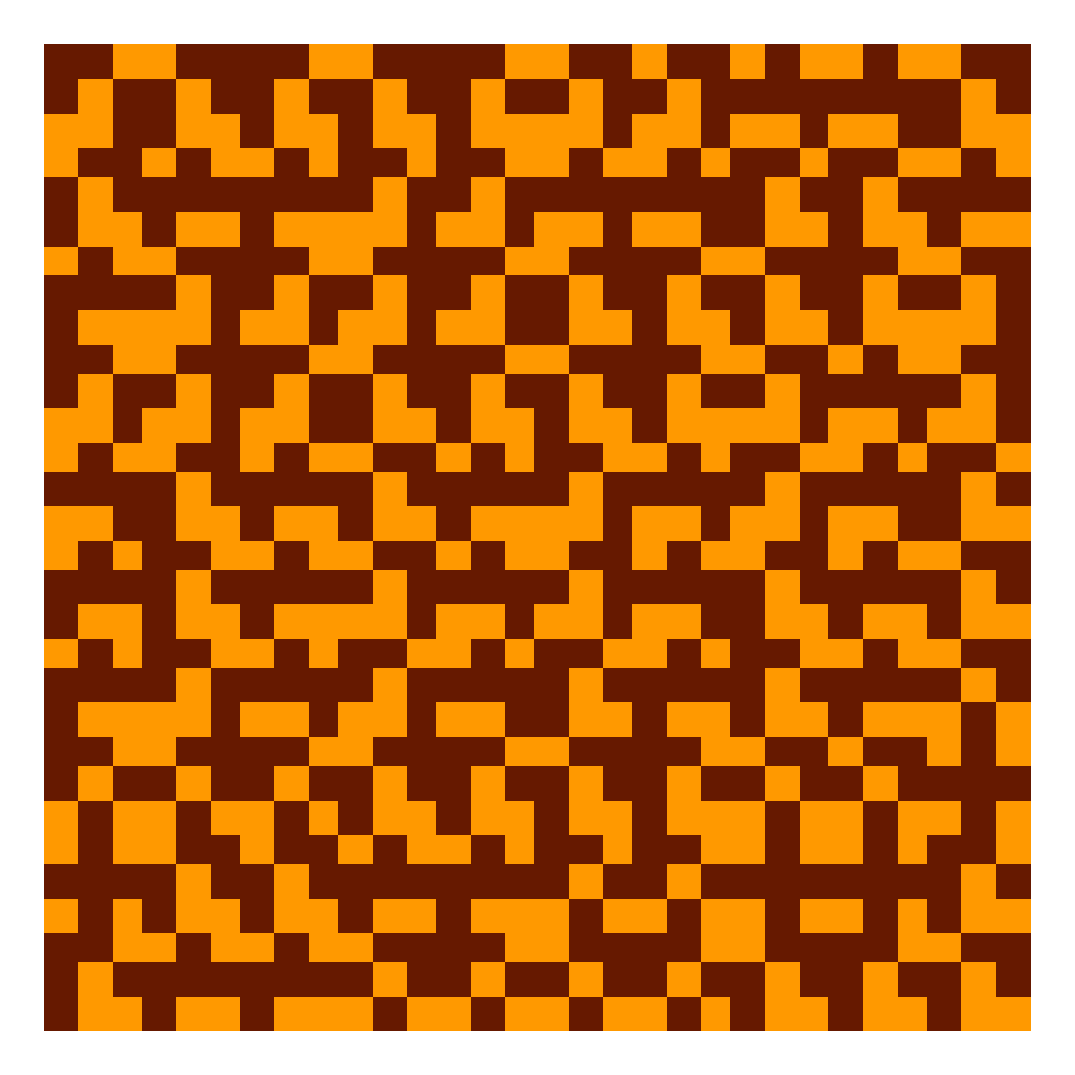
\includegraphics[width=6.2cm]{2005-ae-raster-pe}
&
 \includegraphics[width=6.2cm]{2005-ae-raster-diag}
\\
(a)&(b)&(c) \\
$\;$\\
 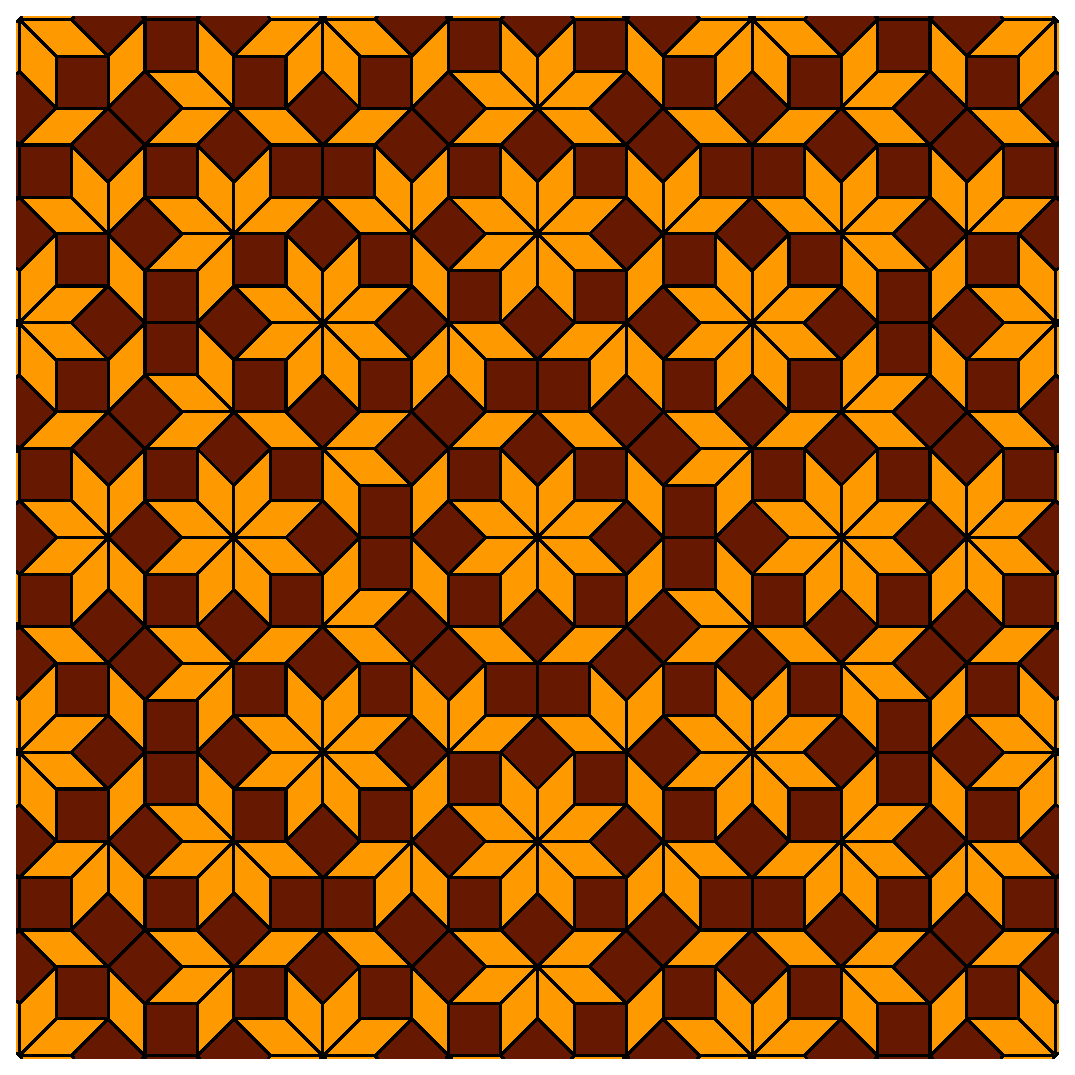
\includegraphics[width=5.87cm]{2005-ae-tiling}
&
 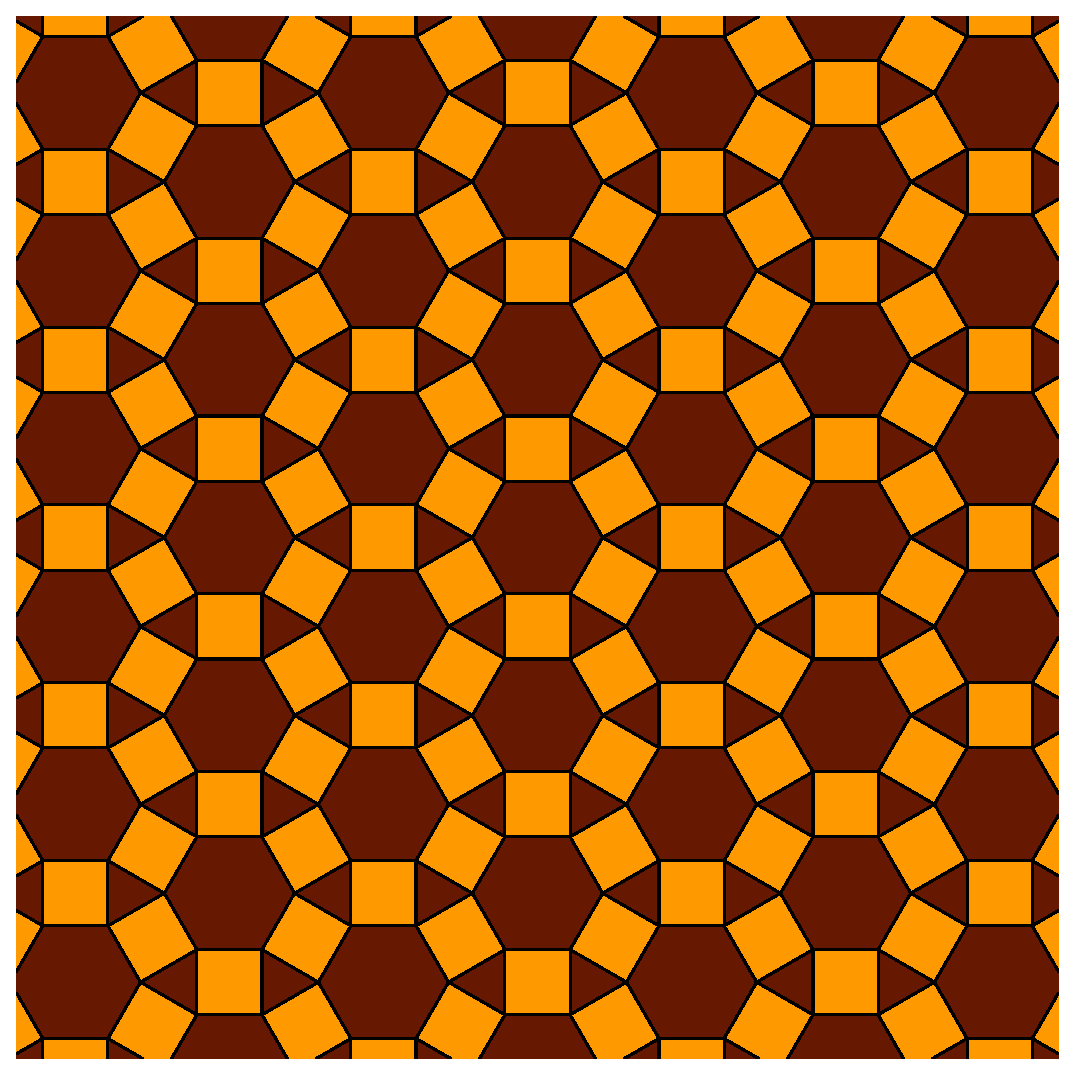
\includegraphics[width=5.87cm]{2005-ae-tess}
&
 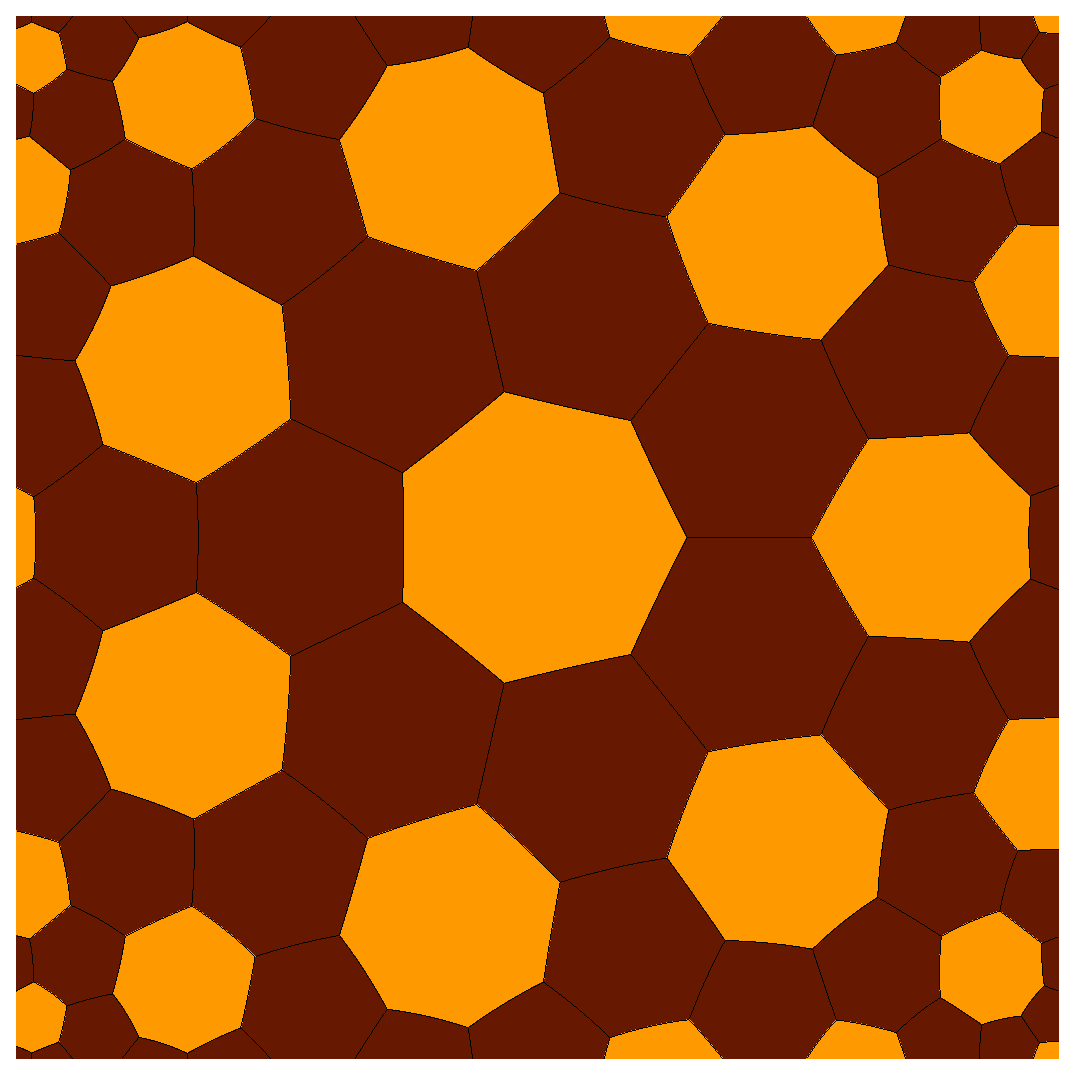
\includegraphics[width=5.87cm]{2005-ae-tess2}
\\
(d)&(e)&(f)\\
$\;$\\
 \includegraphics[width=5.87cm]{2005-ae-tess3}
&
 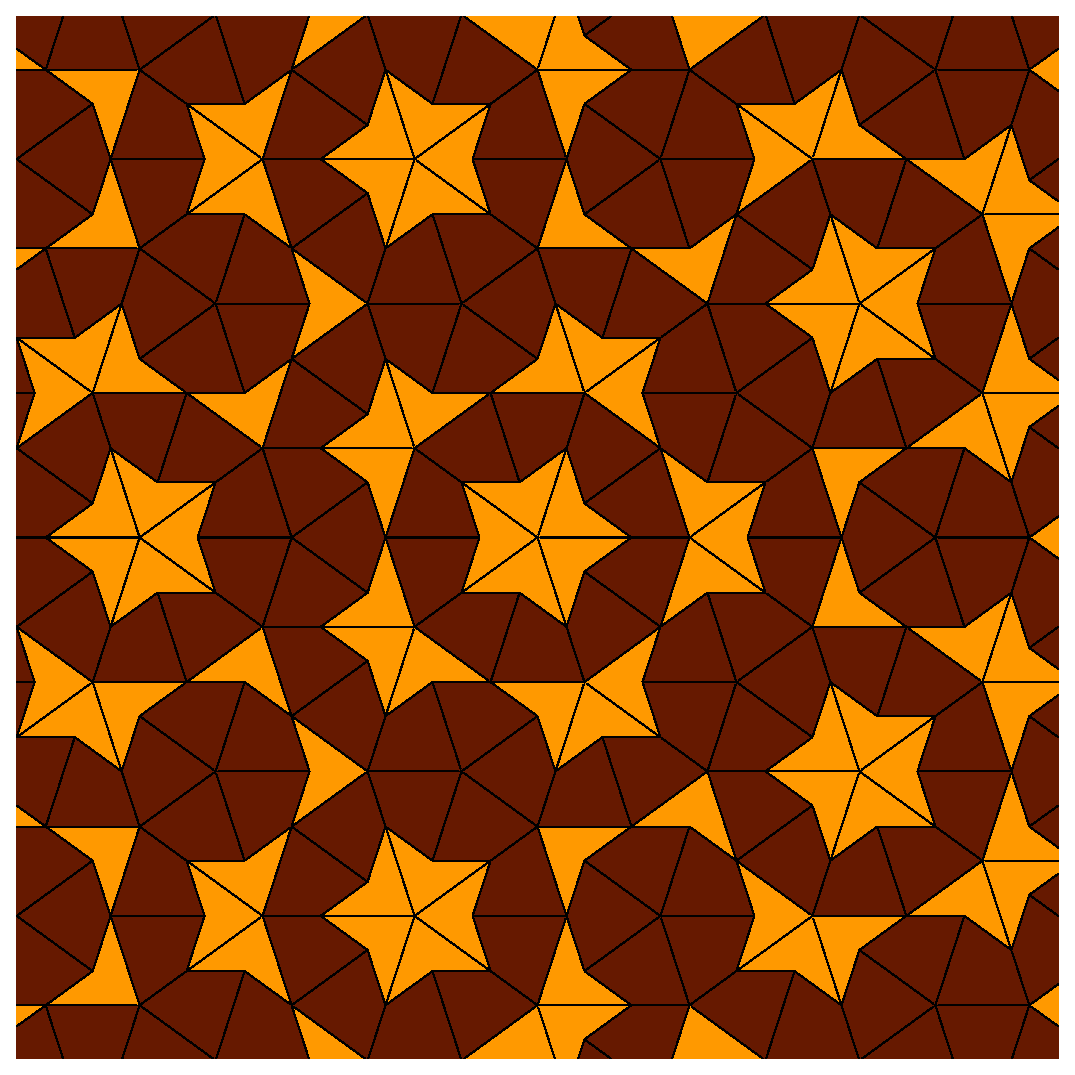
\includegraphics[width=5.87cm]{2005-ae-penrose}
&
 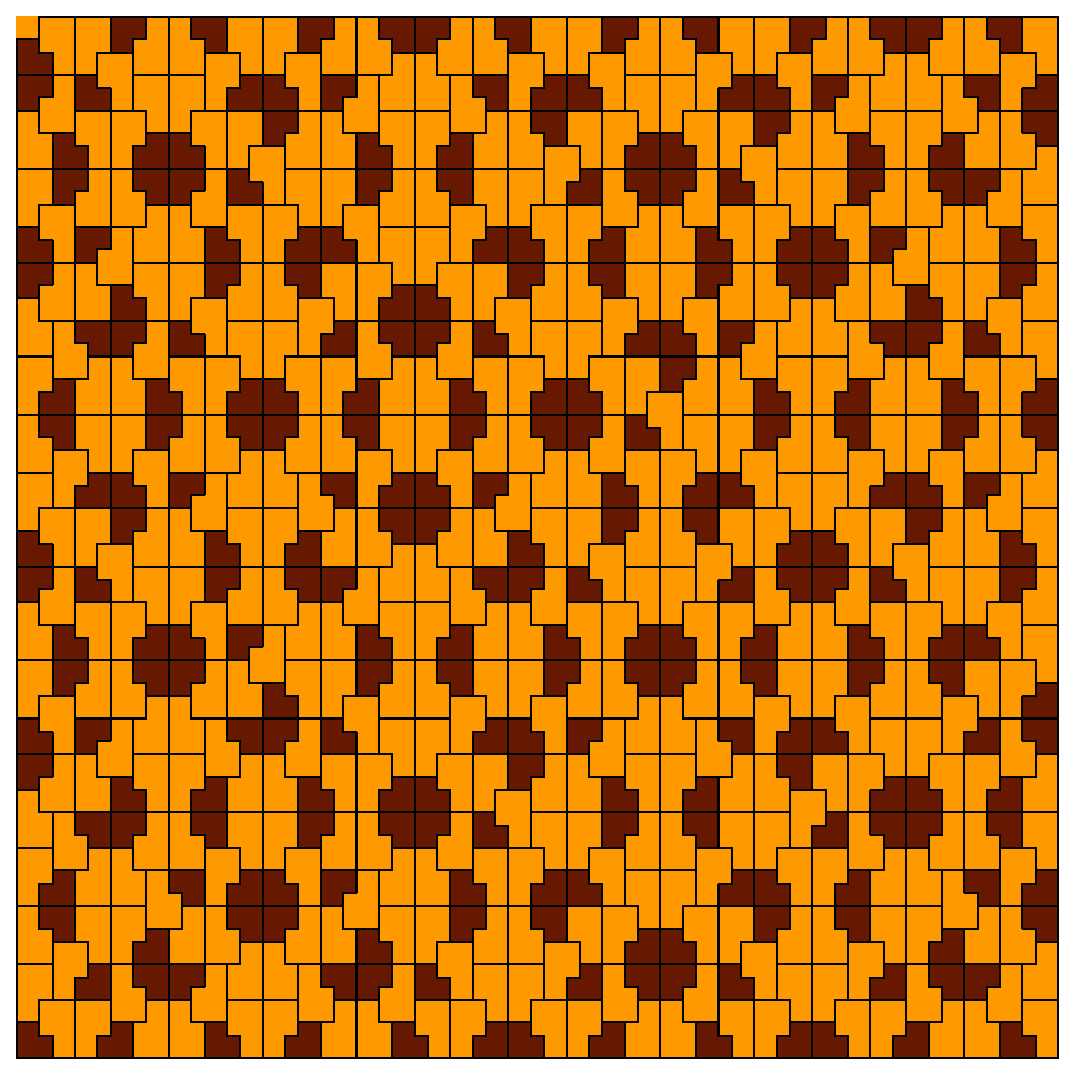
\includegraphics[width=5.87cm]{2005-ae-ammann}
\\
(g)&(h)&(i)\\
\end{tabular}
\end{center}
   \caption{Raster graphics
(a) from white noise;
(b) from permutations in a quantum
and automaton state discrimination problem;
(c) from regular tessellation through repetition;
(d) Tiling obtained from the projection of a dimensional hypercube with
an algorithm by  Grimm and Schreiber;
(e-g) Tilings from
an algorithm by  Sremcevic and Sazdanovic (MathSource 4540);
%http://library.wolfram.com/infocenter/MathSource/4540/
(h) Tiling from
an algorithm by Lyman P. Hurd (MathSource 595);
%http://library.wolfram.com/infocenter/MathSource/595/
(i) Ammann aperiodic tiling from
an algorithm by Sasho Kalajdzievski (MathSource 4273);
%http://library.wolfram.com/infocenter/MathSource/4273/
}
   \label{2005-ae-raster-wn}
 \end{figure}
 }


\frame[shrink=2]{
\frametitle{Parquet flooring}
\begin{figure}
%\centerline{\reserve{19.0cm}{24.5cm}{pdf: image width 19.0cm (2005-ae-parkett.jpg)}}
\centerline{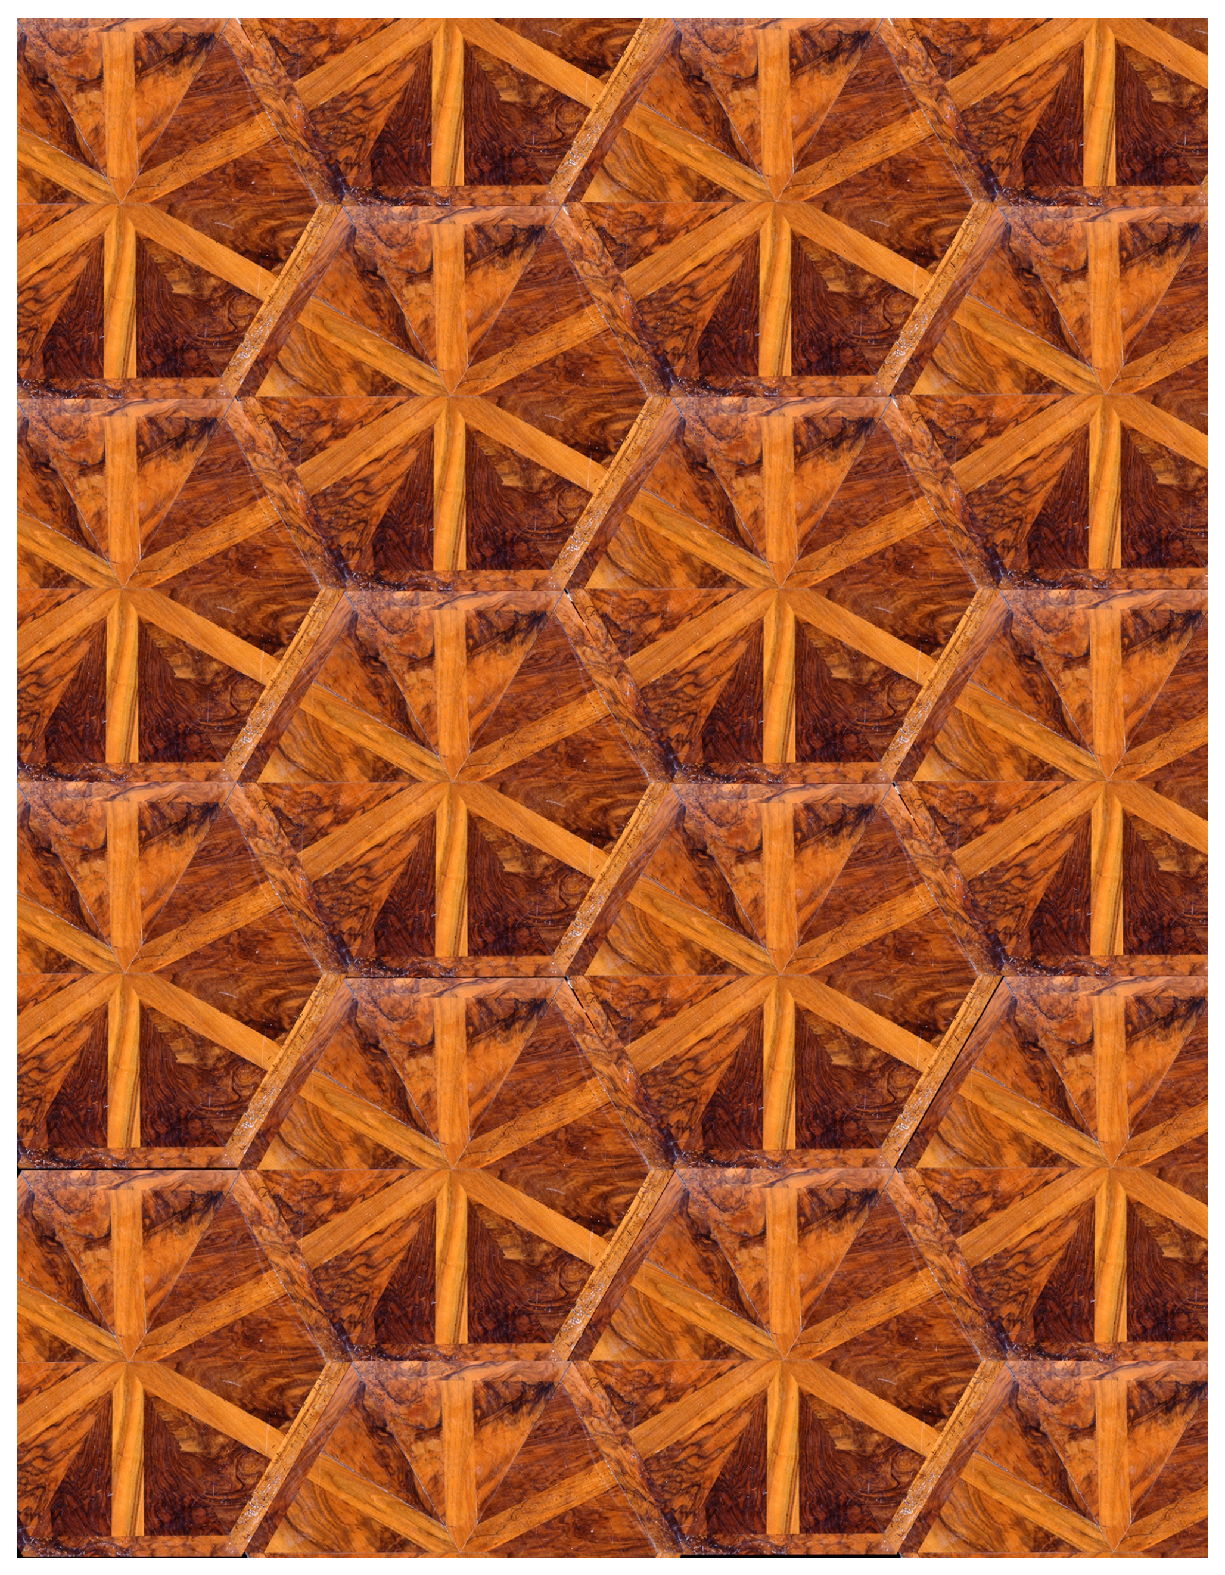
\includegraphics[width=19cm]{2005-ae-parkett}}
   \caption{Parquet flooring  in the galery rooms of the Garden Palais
 Liechtenstein, late 18th century, Vienna, Austria
(\copyright Sammlungen des F\"ursten von und zu Liechtenstein, Vaduz.
URL http://www.liechtensteinmuseum.at)}
   \label{2005-ae-flooring}
 \end{figure}
 }

\frame[shrink=2]{
\frametitle{Wood}
\begin{figure}
%\centerline{\reserve{19.0cm}{19.0cm}{pdf: image width 19.0cm (2005-ae-foliage.jpg)}}
\centerline{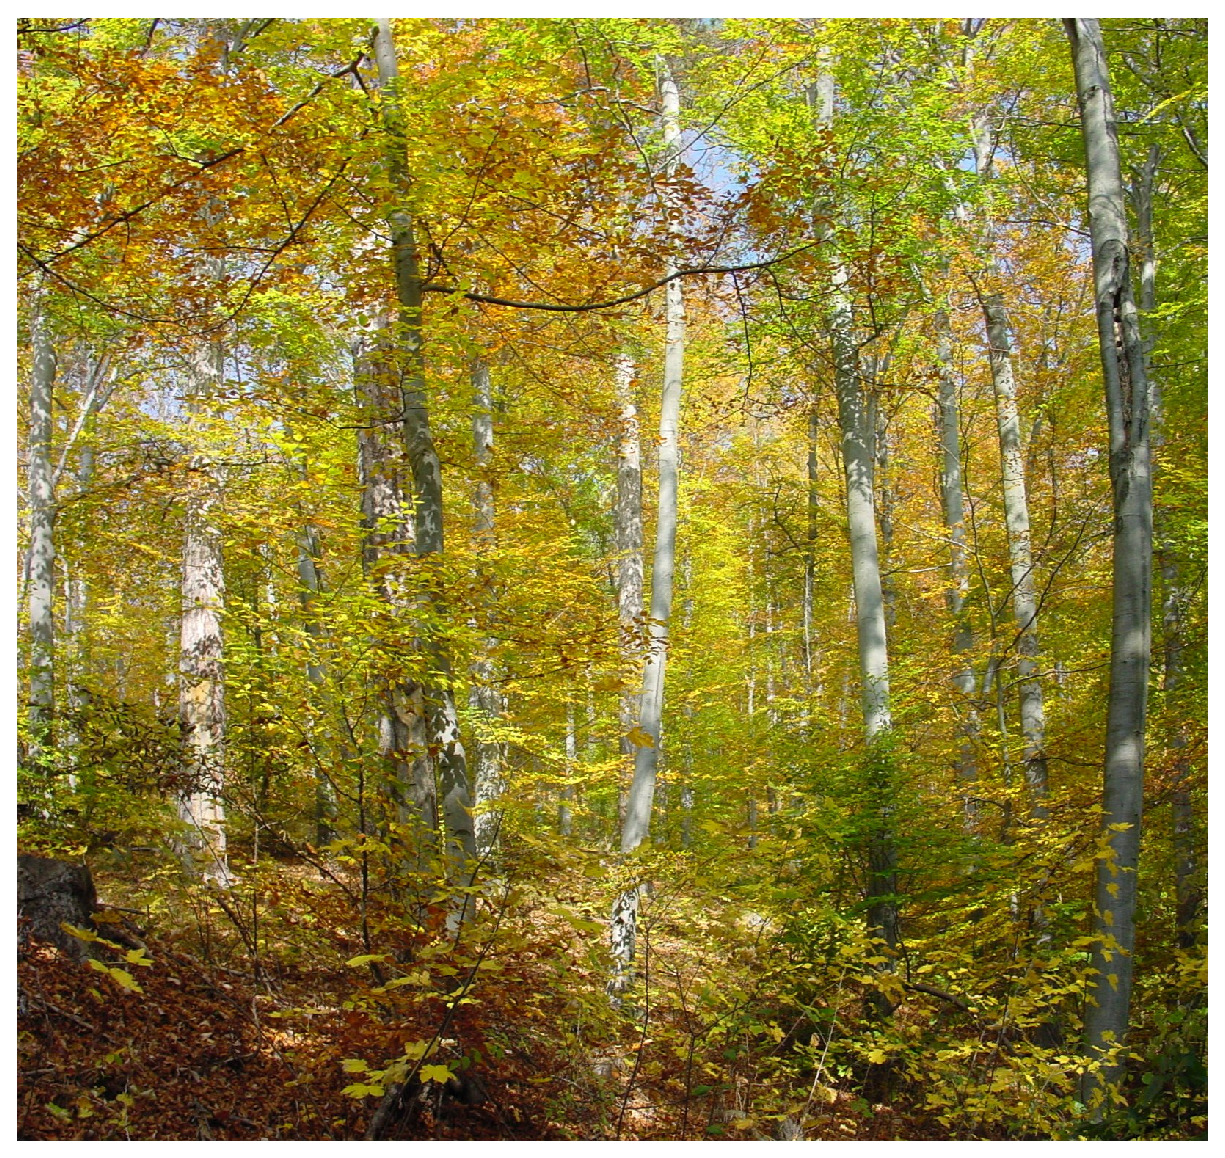
\includegraphics[width=19cm]{2005-ae-foliage}}
  \caption{Autumn foliage near Baden, Lower Austria, Oct. 15, 2000
(\copyright Karl Svozil)}
   \label{2005-ae-foliage}
 \end{figure}
 }


\subsection{One desideratum of VR modelling (among others)}
\frame{
\frametitle{VR marketable as holiday retreat}
VR should be capable of presenting a realistic alternative to
``all inclusive'' holiday resorts.
 }


\end{document}
